\documentclass[12pt]{article}
\usepackage[utf8]{inputenc}
\usepackage{float}
\usepackage{amsmath}
\usepackage{graphicx}

\usepackage{tikz}
\usepackage[hmargin=3cm,vmargin=6.0cm]{geometry}
\topmargin=-2cm
\addtolength{\textheight}{6.5cm}
\addtolength{\textwidth}{2.0cm}
\setlength{\oddsidemargin}{0.0cm}
\setlength{\evensidemargin}{0.0cm}
\usepackage{indentfirst}
\usepackage{amsfonts}

\begin{document}

\section*{Student Information}

Name : Mithat Can Timurcan  \\

ID : 2581064


\section*{Answer 1}
\subsection*{a)}
\begin{itemize}
    \item To find the value of $k$, we need to make sure that the total probability is equal to 1.
    \begin{equation*}
        \begin{split}
            \textbf{P}\{(X,Y) \in A\} = \iint\limits_{(x,y) \in A} f_{X,Y}(x,y)\;dx\;dy = 1 \text{ where } A = [0,1] \times [0,1]
        \end{split}
     \end{equation*}
     \item Which can be written as:
     \begin{equation*}
        \begin{split}
            \iint\limits_{(x,y) \in A} f_{X,Y}(x,y)\;dx\;dy = \int_0^1\int_0^1(x + ky^3)\;dx\;dy = \int_0^1 \left(\frac{x^2}{2} + ky^3x  \right)\Big|_0^1\;dy \\
            = \int_0^1 \left(\frac{1}{2} + ky^3\right)\;dy = \left(\frac{y}{2} + \frac{ky^4}{4}\right) \Big|_0^1 = \left(\frac{1}{2} + \frac{k}{4}\right) = 1
        \end{split}
     \end{equation*}
     \item Solving for $k$ we get:
     \begin{equation*}
        \begin{split}
            \left(\frac{1}{2} + \frac{k}{4}\right) = 1 \rightarrow k = 2
        \end{split}
     \end{equation*}
\end{itemize} 

\subsection*{b)} 
\begin{itemize}
    \item To find the probability of $\textbf{P}\{X = \tfrac{1}{2}\}$, we need to integrate over the joint density function in the following way:
    \begin{equation*}
        \begin{split}
            \textbf{P}\{(X,Y) \in A\} = \iint\limits_{(x,y) \in A} f_{X,Y}(x,y)\;dx\;dy \text{ where } A = \{\tfrac{1}{2}\} \times [0,1]
        \end{split}
    \end{equation*}
    \begin{equation*}
        \begin{split}
            \textbf{P}\{X = \tfrac{1}{2}\} = \textbf{P}\{X = \tfrac{1}{2}, 0 \leq Y \leq 1\} = \int_{0}^{1}\int_{\tfrac{1}{2}}^{\tfrac{1}{2}}(x + 2y^3)\;dx\;dy = 0
        \end{split}
    \end{equation*}
\end{itemize}

\subsection*{c)} 
\begin{itemize}
    \item To find the probability of $\textbf{P}\{0 \leq X \leq \tfrac{1}{2}, 0 \leq Y \leq \tfrac{1}{2}\}$, we need to integrate over the joint density function in the following way:
    \begin{equation*}
        \begin{split}
            \textbf{P}\{(X,Y) \in A\} = \iint\limits_{(x,y) \in A} f_{X,Y}(x,y)\;dx\;dy \text{ where } A =  [0,\tfrac{1}{2}] \times [0,\tfrac{1}{2}]\\
        \end{split}
    \end{equation*}
    \begin{equation*}
        \begin{split}
            \iint\limits_{(x,y) \in A} f_{X,Y}(x,y)\;dx\;dy = \int_{0}^{\tfrac{1}{2}}\int_{0}^{\tfrac{1}{2}}(x + 2y^3)\;dx\;dy = \int_{0}^{\tfrac{1}{2}} \left(\frac{x^2}{2} + 2xy^3  \right)\Big|_{0}^{\tfrac{1}{2}}\;dy \\
            = \int_{0}^{\tfrac{1}{2}} \left(\frac{1}{8} + y^3\right)\;dy = \left(\frac{y}{8} + \frac{y^4}{4}\right) \Big|_{0}^{\tfrac{1}{2}} = \left(\frac{1}{16} + \frac{1}{64}\right) = \frac{5}{64}
        \end{split}
    \end{equation*}
\end{itemize}

\section*{Answer 2}
\subsection*{a)}
\begin{itemize}
    \item In order to find the marginal pdf of $Y$, we need to do the following:
    \begin{equation*}
        \begin{split}
            f_Y(y) = \int_{0}^{\infty} f_{X,Y}(x,y)\;dx = \int_{0}^{\infty} \left(\dfrac{e^{(-y-\tfrac{x}{y})}}{y}\right)\;dx = \dfrac{e^{-y}}{y} \int_{0}^{\infty} e^{-\tfrac{x}{y}}\;dx
        \end{split}
    \end{equation*}
    \begin{equation*}
        \begin{split}
            \dfrac{e^{-y}}{y}\left(-ye^{-\tfrac{x}{y}}\Big|_{0}^{\infty}\right) = \dfrac{e^{-y}}{y} (0 - (-y)) = \dfrac{e^{-y}}{y} \cdot y = e^{-y}
        \end{split}
    \end{equation*}
    \item We can see that $f_Y(y)$ is in the form of $\lambda e^{\lambda y}$ with $\lambda = 1$. Therefore, we can say that our variable $Y$ follows the exponential distribution.
\end{itemize} 

\subsection*{b)} 
\begin{itemize}
    \item We can find the expected value of $Y$ with the following formula:
    \begin{equation*}
        \begin{split}
            \textbf{E}(Y) = \mu_Y = \int_{0}^{\infty} yf_{Y}(y)\;dy = \int_{0}^{\infty} ye^{-y}\;dy
        \end{split}
    \end{equation*}
    \item We also know that if a variable follows the exponential distribution, it's expected value can be computed using the $\lambda$ value:
    \begin{equation*}
        \begin{split}
            \textbf{E}(Y) = \mu_Y = \dfrac{1}{\lambda}
        \end{split}
    \end{equation*}
    \item Since we've found the $\lambda$ value as 1, we can see that our expected value of $Y$, $\textbf{E}(Y)$ is equal to 1.
\end{itemize}


\section*{Answer 3}
\subsection*{a)}
\begin{itemize}
    \item We can use binomial distribution in this problem. Since we know that $10\%$ of the soldiers belong to the naval forces, we can take the success value $p$ as 0.1. We want to make sure that $9\%$ of the 1000 soldiers belong to the naval forces so there should be at least 90 soldiers. We can calculate this in the following way:
    \begin{equation*}
        \begin{split}
            \textbf{P}\{X \geq 90\} = 1 - \textbf{P}\{X \leq 89\} = 1 - \sum_{k = 0}^{89} \begin{pmatrix} 1000 \\ k \end{pmatrix} p^k(1-p)^{1000-k} \approx 0.867\\
            \text{calculated using the binocdf function on octave.}
        \end{split}
     \end{equation*}
     \item We also know that for large values of $n$ and moderate values of $p$, Normal distribution tends to approximate Binomial distribution with the mean of $\mu = np$ and standard deviation of $\sigma = \sqrt[]{np(1-p)}$. However, we also need to apply continuity correction since we're approximating a discrete distribution by a continuous distribution so we're going to expand our interval by 0.5 units, making it 89.5. Then we can use the \texttt{normcdf($x$, $\mu$, $\sigma$)} on Octave.
     \begin{equation*}
        \begin{split}
            \textbf{P}\{X \geq 90\} = 1 - \textbf{P}\{X \leq 89.5\}\\ 1 - \texttt{normcdf(89.5, 1000*0.1, sqrt(1000*0.1*0.9))} \approx 0.866\\
        \end{split}
     \end{equation*}
\end{itemize} 

\subsection*{b)}
\begin{itemize}
    \item We can use the same approach we used in part a). However, this time our pool consists of 2000 soldiers so we need to make sure that there are at least 180 that belong to the naval forces. We can achieve this in the following way:
    \begin{equation*}
        \begin{split}
            \textbf{P}\{X \geq 180\} = 1 - \textbf{P}\{X \leq 179\} = 1 - \sum_{k = 0}^{179} \begin{pmatrix} 2000 \\ k \end{pmatrix} p^k(1-p)^{2000-k} \approx 0.939\\
            \text{calculated using the binocdf function on octave.}
        \end{split}
     \end{equation*}
     \item We can also use Normal approximation to Binomial like we did in the previous part:
     \begin{equation*}
        \begin{split}
            \textbf{P}\{X \geq 180\} = 1 - \textbf{P}\{X \leq 179.5\}\\ 
            1 - \texttt{normcdf(179.5, 2000*0.1, sqrt(2000*0.1*0.9))} \approx 0.937\\
        \end{split}
     \end{equation*}
     \item According to the Central Limit Theorem, as the sample size increases, the distribution of the sample proportion approaches a normal distribution. Consequently, the variability in the proportion of naval soldiers across various samples diminishes with larger sample sizes. This reduced variability increases the likelihood of consistently meeting or surpassing the minimum percentage requirement.
\end{itemize}


\section*{Answer 4}
\subsection*{a)}
\begin{itemize}
    \item First of all, we should standardize our variable, (let us denote with $T$) with a mean $\mu$ of 65 years and a standard deviation $\sigma$ of 6 years:
    \begin{equation*}
        \begin{split}
            \textbf{P}\{60 < T < 75\} = \textbf{P}\left\{\dfrac{60-\mu}{\sigma} < \dfrac{T-\mu}{\sigma} < \dfrac{75-\mu}{\sigma} \right\} \\
            \textbf{P}\left\{\dfrac{60-65}{6} < Z < \dfrac{75-65}{6} \right\} = \textbf{P}\{-0.833 < Z < 1.667\}\\
            \Phi(1.667) - \Phi(-0.833) \approx 0.750 \\
            \text{calculated using the normcdf function on octave.}
        \end{split}
     \end{equation*}
\end{itemize} 

\subsection*{b)}
\begin{figure}[H]
    \centering
    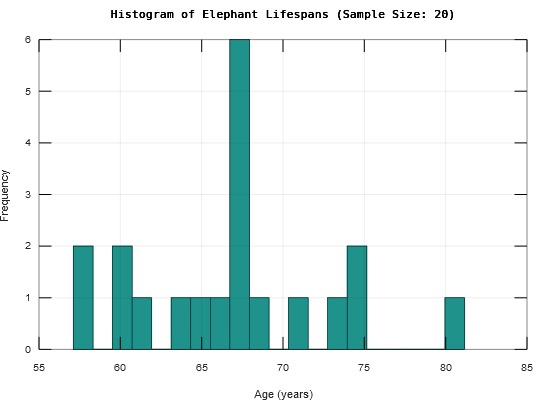
\includegraphics[width=0.65\textwidth]{plots/plot for 20.jpg}
    \caption{Histogram when the sample size is 20.}
    \label{fig:example_b}
\end{figure}
\begin{figure}[H]
    \centering
    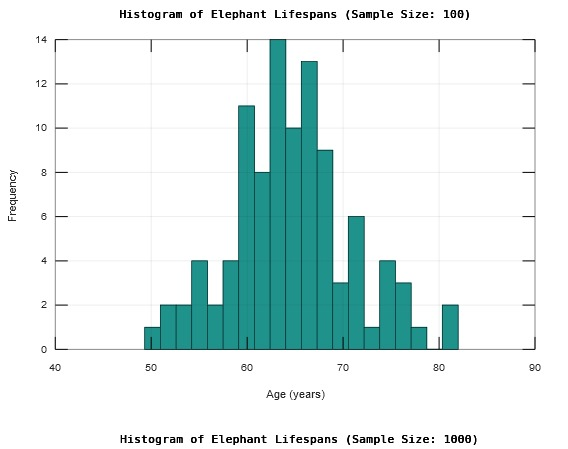
\includegraphics[width=0.65\textwidth]{plots/plot for 100.jpg}
    \caption{Histogram when the sample size is 100.}
\end{figure}
\begin{figure}[H]
    \centering
    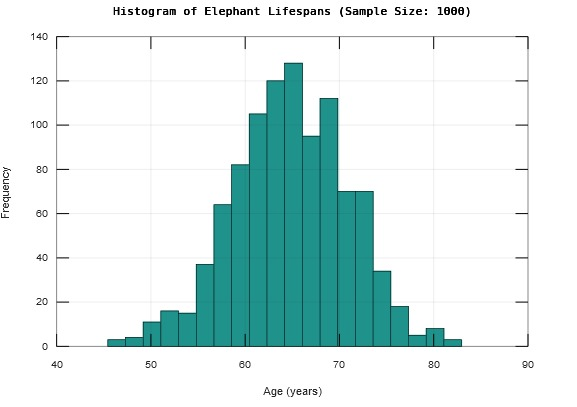
\includegraphics[width=0.65\textwidth]{plots/plot for 1000.jpg}
    \caption{Histogram when the sample size is 1000.}
\end{figure}

\begin{itemize}
    \item These histograms verify our knowledge that as the sample size increases, the distribution of
    the sample proportion approaches a normal distribution according to the Central Limit Theorem.
\end{itemize}

\begin{figure}[H]
    \centering
    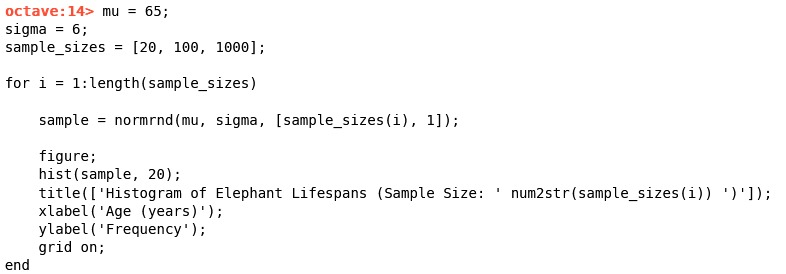
\includegraphics[width=0.7\textwidth]{plots/octave code for the plots.jpg}
    \caption{Octave/Matlab code for the plots.}
\end{figure}

\subsection*{c)}
\begin{figure}[H]
    \centering
    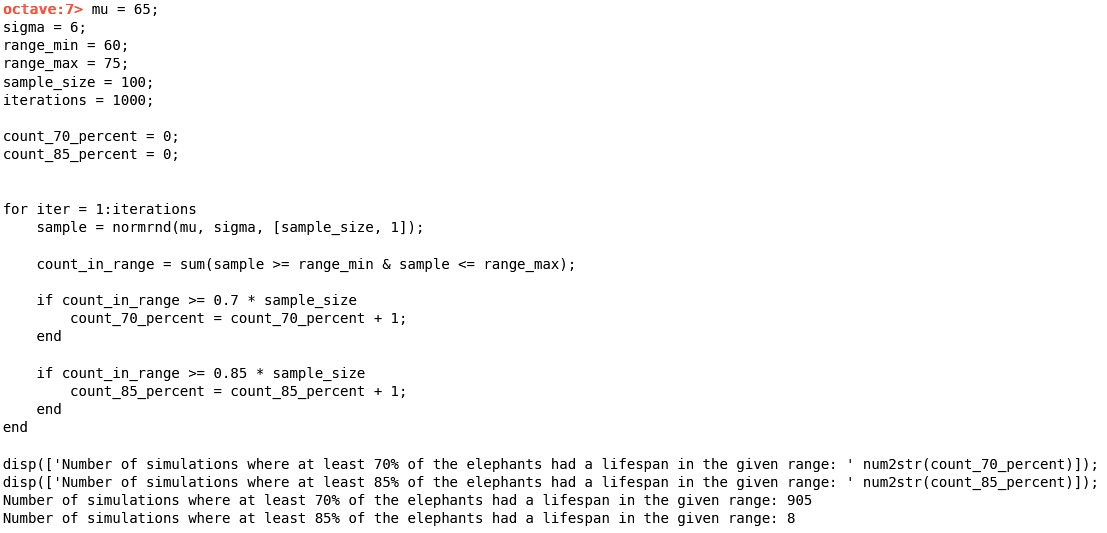
\includegraphics[width=0.9\textwidth]{plots/4c code output.jpg}
    \caption{Octave/Matlab code and the output for the simulations.}
\end{figure}

\begin{itemize}
    \item In part a), we found that approximately $75\%$ of the elephants will live more than 60 years, but less than 75 years. Looking to our simulations, in 905 of them, we observe at least $70\%$ of elephants having a lifespan in the given range. This result aligns closely with our expected percentage of $75\%$. It suggests that our model's predictions are consistent with reality in this case. However, in only 8 of the simulations, we observe that at least $85\%$ of the elephants having a lifespan in the given range. This result is significantly lower than our expected percentage of $75\%$. It indicates that such a high concentration of elephants within the specified age range is less likely to occur based on our model's predictions.
\end{itemize}

\end{document}




